\uuid{65GE}
\niveau{PCSI}
\module{Analyse}
\chapitre{Généralités sur les fonctions}
\sousChapitre{Equations, inéquations}
%!TeX root=../../../encours.nouveau.tex
%%% Début exercice %%%

\duree{10}
\difficulte{1}
\auteur{Antoine Crouzet}
\datecreate{01/12/2024}
\titre{Des inégalités sympathiques}
\contenu{
\question{Démontrer les inégalités suivantes :
\[ \forall~x\in \R,\, \eu{x}\geq 1+x,\quad \forall~x\in \interff{0 \frac{\pi}{2}},\, \sin(x)\geq \frac{2x}{\pi} \]}
\reponse{Posons $f$ la fonction définie sur $\R$ par $f:x\mapsto \eu{x}-1-x$. $f$ est dérivable sur $\R$ (exponentielle et polynôme) et on
\begin{align*}
  \forall~x\in \R,\, f'(x) &= \eu{x}-1
\end{align*}
Remarquons que $f'(x)\geq 0 \Longleftrightarrow \eu{x}\geq 1 \Longleftrightarrow x \geq 0$ par stricte croissance d'exponentielle. On obtient alors le tableau de variations de $f$ suivant :
\begin{center}
  \begin{tikzpicture}
   \tkzTabInit{$x$ / 0.7 , $f'(x)$ / 0.7, $f$ / 1.1}{$-\infty$, $1$, $+\infty$}
   \tkzTabLine{, -, z, +, }
   \tkzTabVar{+/ , -/0 , +/ }
\end{tikzpicture}
\end{center}
On en déduit ainsi que $0$ est un minimum de $f$, et donc \[ \boxed{\forall x\in \R,\, \eu{x}-1-x\geq 0 \Longleftrightarrow \eu{x}\geq 1+x}. \]

De même, posons $g$ la fonction définie sur $\left] 0,\,\dfrac{\pi}{2}\right[$ par $g:x\mapsto \sin(x)-\frac{2x}{\pi}$. $g$ est dérivable sur son domaine de définition (comme somme de $\sin$ et de fonction affine) et on a \[ \forall x\in \interoo{0 \dfrac{\pi}{2}},\, g'(x) = \cos(x)-\frac{2}{\pi} \]
$g'$ est à nouveau dérivable pour les mêmes raisons, et on a
\[ \forall x\in \interoo{0 \dfrac{\pi}{2}},\, g''(x) = -\sin(x) \]
$g'$ est donc négative sur $\left] 0,\,\dfrac{\pi}{2}\right[$. On en déduit le tableau de variations de $g'$ suivant :
\begin{center}
  \begin{tikzpicture}
   \tkzTabInit{$x$ / 0.7 , $g''(x)$ / 0.7, $g'$ / 1.1}{$0$,  $\frac{\pi}{2}$}
   \tkzTabLine{, -, }
   \tkzTabVar{+/$1-\frac{2}{\pi}$ ,  -/ $-\frac{2}{\pi}$}
\end{tikzpicture}
\end{center}
$g'$ est continue sur $\left] 0,\,\dfrac{\pi}{2}\right[$ et est strictement décroissante. Puisque $g'(0)=1-\frac{2}{\pi}>0$ et $g'\left(\frac{\pi}{2}\right)=-\frac{2}{\pi}<0$, d'après le théorème de la bijection, il existe un unique $a\in \left]0,\,\dfrac{\pi}{2}\right[$ tel que $g'(a)=0$. On peut alors écrire :
\begin{center}
  \begin{tikzpicture}
   \tkzTabInit{$x$ / 0.7 , $g'$ / 1.1, $g'(x)$ / 0.7, $g$ / 1.1}{$0$, $a$ , $\frac{\pi}{2}$}
   \tkzTabVar{+ / $1-\frac{2}{\pi}$ , R/,  -/ $-\frac{2}{\pi}$}
   \tkzTabIma{1}{3}{2}{$0$}
   \tkzTabLine{, +, z, -,}
   \tkzTabVar{ - / $0$, +/$g(a)$, -/$0$}
\end{tikzpicture}
\end{center}
Ce qui nous permet de conclure que, pour tout $x\in \left] 0,\,\dfrac{\pi}{2}\right[$, $g(x)\geq 0$, ce qui donne le résultat.}
}

%%% Fin exercice %%%
